\begin{frame}[fragile]{Crews Module}
    \texttt{./src/emergency\_planner/crews/}
    \begin{columns}[T]
      \begin{column}{0.3\textwidth}
          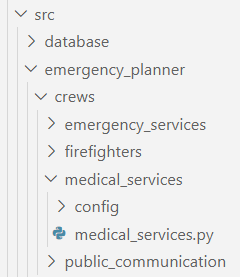
\includegraphics[width=\textwidth]{figures/crews_modules_folders.png}
      \end{column}
      \begin{column}{0.68\textwidth}
        \texttt{medical\_services.py}
        \begin{lstlisting}[language=Python, breaklines=true]
@CrewBase
class MedicalServicesCrew:
    """Medical Services Crew"""
    @agent
    def medical_services_operator(self) -> Agent:
        return Agent(config=self.agents_config["medical_services_operator"])
        ...
    @task
    def fetch_hospital_information(self) -> Task:
        config = add_schema_to_task_config(
            self.tasks_config["fetch_hospital_information"],
            HospitalsInformation.model_json_schema(),
        )
        return Task(config=config, tools=[hospital_reader_tool])
        \end{lstlisting}
      \end{column}
    \end{columns}
\end{frame}